\documentclass[10pt,letterpaper]{article}
\usepackage[margin=0.8in]{geometry}
\usepackage{times,graphicx,amsmath,amssymb,booktabs,microtype,float}
\usepackage[colorlinks,allcolors=blue]{hyperref}
\title{Task Information Audits for Connectome Graph Interventions\\\large Supplementary Material}
\author{Anonymous}
\date{}
\begin{document}
\maketitle

\section{Source visibility and population solvability}

\paragraph{Audit outputs and path accounting.}
The inputs are an edited graph, its fixed linear propagator, source nodes,
readout nodes and a task statement. Structural validation first checks the
invariants declared by the intervention. The transfer $T=R_SW^2E_{ab}$ is
computed by sparse propagation of source basis vectors. The audit reports
nonzero source columns (access), rank (linear source separation), and
column gains and mixing geometry. For the specified subspace XOR,
Proposition~1 adds the exact ideal Bayes decision. Finite readouts are
reported separately rather than used to redefine source information.

With incoming-neighbor normalization, each transfer entry expands as
$T_{sj}=\sum_r W_{sr}W_{rj}$. A common-relay triple restricts this sum
to a relay receiving both sources. Removing every such triple does not
remove terms with distinct relays. Equal $T$ implies identical readout
inputs for any source features under the fixed operator; equal structural
counts do not.

\paragraph{Private transfer component.}
For multiple active sources, write $t_j=T_{:j}$ and let $T_{-j}$ contain
the other columns. Using the Moore--Penrose pseudoinverse,
$q_j=t_j-T_{-j}T_{-j}^{+}t_j$ and $\rho_j=\|q_j\|_2^2$. This is the
squared residual after least-squares projection onto the other transfer
columns. It is zero for a deleted source and also for a source whose
transfer is collinear with other sources. It is a property of the
executed linear operator, not an information-theoretic necessity
condition for all visual tasks.

Recomputing this quantity from the saved graph arrays for source 109
gives $\rho_{109}=0$, $0.001953125$, and $0$ on the base, named-edge
zero and path-zero graphs. For source 107, all three residuals are zero.
The named-edge matrix has columns $(0,0.125,0.0625,0.0625)^\top$ and
$(0.0625,0.125,0.0625,0.0625)^\top$ at its two rows, in source order
$(109,107,152,6)$. Its source-109 residual is $(-0.03125,0.03125)$.
The base and path-zero source-109 columns are collinear with source 6.
These are deterministic checks of archived graph arrays, not new
model evaluations.

For adjacency $A_{uv}=1$ encoding $u\to v$, our main propagator is
$W_{vu}=A_{uv}/\max(d_v,1)$, with $d_v=\sum_u A_{uv}$.
Nonzero features are present only at the two designated sources.
Writing their stacked features as $X_{ab}$, the sink features after two
linear propagation rounds are exactly
\[
 H_S=R_SW^2E_{ab}X_{ab}=T(A)X_{ab}.
\]
Source visibility means a nonzero column of $T$. For the ideal noiseless
subspace task it exactly characterizes Bayes solvability. Assume independent
balanced source classes $c_a,c_b$, independent
$z_a,z_b\sim\mathcal N(0,I_8)$, source vectors $x_j=P_{c_j}z_j$,
and $U_0\cap U_1=\{0\}$ for $U_c=\operatorname{span}(P_c)$.
The fixed transfer $T$ is nonnegative, and all other node inputs are zero.

If, for example, $T_{:b}=0$, $H_S$ is independent of $c_b$.
Conditioning on any value of $H_S$ and on $c_a$ leaves $c_b$ balanced.
Consequently $\Pr(c_a\oplus c_b=1\mid H_S)=1/2$, and Bayes
accuracy is exactly $1/2$.

If both columns are nonzero, form the measurable sink sum
\[
 z=\sum_{s\in S}(H_S)_s=\alpha x_a+\beta x_b,\qquad
 \alpha=\sum_sT_{sa}>0,\quad\beta=\sum_sT_{sb}>0.
\]
For $c_a=c_b=c$, both terms lie in $U_c$, so $z\in U_0\cup U_1$.
For $c_a\ne c_b$, suppose $z\in U_{c_a}$. Subtracting
$\alpha x_a\in U_{c_a}$ implies $\beta x_b\in U_{c_a}\cap U_{c_b}$,
which forces $x_b=0$. Independent nondegenerate Gaussian coordinates
make this a probability-zero event. The same argument excludes membership
in $U_{c_b}$. Thus
$y=\mathbf 1\{z\notin U_0\cup U_1\}$ almost surely, proving Bayes
accuracy one.

Independent random eight-dimensional class subspaces in $\mathbb R^{16}$
are transverse with probability one. Regenerating the ten original
seed-specific basis recipes gives numerical rank 16 for every
concatenated matrix $[P_0\ P_1]$. The result concerns exact, noiseless
population information; it gives no convergence or generalization rate
for the finite MLP, and subspace membership is not a finite-precision or
noise-robust decoding guarantee.

The common-relay predicate is narrower. Consider six nodes with edges
$a\to r_a\to s_1$ and $b\to r_b\to s_2$, with distinct relays. There
are no common-relay triples, but the source-to-sink matrix is
\[
 T=\begin{pmatrix}1&0\\0&1\end{pmatrix}.
\]
The concatenated readout sees both source vectors and can learn their
classes and XOR. Thus zero common-relay triples does not certify that
all task information is absent. This counterexample is an exact matrix
check, not an additional trained experiment.

On the 96-node controlled graph, the situation is different by design.
The two source nodes have only one outgoing edge each, both to the
designated relay, and neither sink has another incoming edge. Its source
transfer matrix is
$T=\left(\begin{smallmatrix}.5&.5\\.5&.5\end{smallmatrix}\right)$;
removing the four motif edges gives $T=0$. The graph has 337 edges,
including background edges outside these protected destinations. The
tiny checks in \texttt{analysis/check\_operator\_semantics.py} reconstruct
this graph and verify both matrices using local Apple MPS, without
training. These controlled-graph checks are separate from the real-graph reconstruction below.

\section{Intervention implementation}

The path family contains pairs $(r,s)$ with
$a\to r$, $b\to r$, and $r\to s$, for $s$ among the two fixed sinks.
It is enumerated in ascending relay/sink order. The retained set $K_q$
is a prefix of this order. Since triples share source edges, we operate
on the union of path edges rather than independently deleting each
triple. Edges belonging to retained triples are protected.

For each edge to remove, the implementation shuffles the list of
module-matched partner edges and accepts the first feasible directed
double-edge exchange. Each exchange preserves the degree of every
labeled node algebraically: both source out-degrees and both target
in-degrees retain one edge. Matching the two source-module labels and
the two target-module labels also preserves module-pair counts. The
runtime records compare degree sequences and module counts and assert
the terminal common-relay set. The primitive additionally forbids
self-loops, duplicate edges, direct source-to-sink edges, the recreation
of original path edges, and the use of a protected path edge as a partner.
It rejects a candidate if the enumerated family acquires a new member.

This is a constrained editing procedure with randomized partner order.
It is not an MCMC sampler with a demonstrated stationary distribution,
and no claim of uniform null sampling is made. A dose is marked
infeasible if a required removal has no admissible partner; it is not
silently relaxed or assigned a chance score. All reported path doses
in these cohorts were feasible in the original records.

The subsequent degree and protected nulls have a different role. Their
swap chains randomize the dose graph, optionally keeping the selected
path-edge union fixed, without the no-new-triple constraint. Consequently
the horizontal dose labels in the main figure do not state the final
number of triples in a null graph. The broad zero-dose null successes
are a direct reason to retain that distinction.

\section{Reconstructed real-graph operators}

The public weight table was recovered and its full byte count and SHA-256
matched the recorded release. Rebuilding the dense base NPZs for the broad
and narrow extractions reproduced the frozen hashes byte-for-byte. The
narrow base also reproduces the initial $k=4$ extraction's node/role
metadata. All dose graphs below are deterministic post-hoc replays of
archived code; original dose-instance hashes were not recorded, so these
are not described as saved inputs from the old trained fits.

For the initial narrow extraction, the audit finds
\[
16T_{\rm base}=\begin{pmatrix}2&1\\2&1\end{pmatrix},\quad
16T_{\rm edge0}=\begin{pmatrix}1&0\\1&1\end{pmatrix},\quad
16T_{\rm path0}=\begin{pmatrix}1&0\\1&0\end{pmatrix}.
\]
Both zero-dose reconstructions contain no common-relay triples. Source
$a$ retains routes through compact relay index 18 to both sinks; the
named-edge zero dose additionally retains $b\to57\to s_2$. The
path-conditioned zero dose has no two-hop route from $b$ to either sink.
The surviving separate-relay routes make it inappropriate to attribute
the two conditions' historical accuracy difference to their common-relay
count, which is the same, or uniquely to the no-new-triple rejection rule.
Complete route lists and the individual compensating swaps are supplied
in the reconstructed-graph report.

\begin{table}[H]\centering
\caption{Source-to-readout transfer of the reconstructed $k=8$ dose graphs.
The matrix entries shown are $64T$, with source columns $(a,b)$ and sink
rows $(s_1,s_2)$. A listed source is observable in the structural sense of
having a nonzero column, not guaranteed finite-trained accuracy.}
\small
\begin{tabular}{llcc}\toprule
Extraction & Retained triples & $64T$ & Observable sources\\\midrule
Broad & 0 & $\left(\begin{smallmatrix}0&0\\1&0\end{smallmatrix}\right)$ & $a$\\[5pt]
Broad & 1 & $\left(\begin{smallmatrix}1&1\\1&0\end{smallmatrix}\right)$ & $a,b$\\[5pt]
Broad & 2 & $\left(\begin{smallmatrix}1&1\\2&1\end{smallmatrix}\right)$ & $a,b$\\[5pt]
Broad & 3 & $\left(\begin{smallmatrix}2&2\\2&1\end{smallmatrix}\right)$ & $a,b$\\[5pt]
Narrow & 0 & $\left(\begin{smallmatrix}0&0\\0&0\end{smallmatrix}\right)$ & none\\[5pt]
Narrow & 1 & $\left(\begin{smallmatrix}1&1\\0&0\end{smallmatrix}\right)$ & $a,b$\\[5pt]
Narrow & 2 & $\left(\begin{smallmatrix}1&1\\1&1\end{smallmatrix}\right)$ & $a,b$\\[5pt]
Narrow & 3 & $\left(\begin{smallmatrix}2&2\\1&1\end{smallmatrix}\right)$ & $a,b$\\
\bottomrule\end{tabular}
\end{table}

The base and all three nonzero narrow doses have rank-one transfer
matrices, yet both sources are visible. All nonzero broad and narrow
doses therefore have Bayes accuracy one in the ideal task. Their
different finite-readout accuracies concern the learnability of these
mixtures under the recorded protocol.

\section{Complete accuracy matrices}

All cells report the original mean accuracy and percentile bootstrap
95\% interval over ten seed blocks. The no-cross-node control is $W=I$,
not a zero matrix. Sources and sinks are distinct, so it prevents source
signals from reaching the readout. The edge-deletion control removes the
named motif edges in the first table and the declared common-relay path
edge union in the path-conditioned tables, without degree compensation.
The matrices are generated directly from the supplied JSON copies.
At zero dose, the declared edge set is already absent, so the edge-deletion
column is another readout fit on the same graph, not an additional graph
intervention. Small differences between those fits, including the initial
$k=4$ zero-dose scores 0.9745 and 0.9756, reflect the archived initialization
sequence discussed below. They must not be interpreted as effects of deleting
an edge twice.

\begin{table}[H]\centering
\caption{Named-edge intervention on the narrow $k=4$ extraction. Dose is the requested number of retained named edges, not an assertion of complete functional-path removal. Mean accuracy with original ten-seed-block bootstrap 95\% intervals.}\label{tab:edge-full}
\small\setlength{\tabcolsep}{4pt}
\begin{tabular}{lccccc}\toprule
Dose & Dose graph & No cross-node & Degree null & Protected null & Edge deletion \\ \midrule
0 edges & \shortstack{0.9745\\{}[0.9669,0.9812]} & \shortstack{0.5017\\{}[0.4944,0.5111]} & \shortstack{0.5017\\{}[0.4945,0.5114]} & \shortstack{0.5017\\{}[0.4945,0.5110]} & \shortstack{0.9756\\{}[0.9675,0.9831]} \\[3pt]
1 edge & \shortstack{0.5051\\{}[0.4962,0.5147]} & \shortstack{0.5017\\{}[0.4946,0.5111]} & \shortstack{0.5017\\{}[0.4946,0.5112]} & \shortstack{0.5017\\{}[0.4944,0.5109]} & \shortstack{0.5051\\{}[0.4963,0.5149]} \\[3pt]
2 edges & \shortstack{0.5051\\{}[0.4965,0.5148]} & \shortstack{0.5017\\{}[0.4945,0.5112]} & \shortstack{0.5017\\{}[0.4945,0.5109]} & \shortstack{0.5017\\{}[0.4945,0.5109]} & \shortstack{0.5051\\{}[0.4965,0.5146]} \\[3pt]
4 edges & \shortstack{0.9772\\{}[0.9727,0.9820]} & \shortstack{0.5017\\{}[0.4943,0.5108]} & \shortstack{0.5017\\{}[0.4945,0.5109]} & \shortstack{0.9794\\{}[0.9745,0.9836]} & \shortstack{0.5004\\{}[0.4929,0.5102]} \\[3pt]
\bottomrule\end{tabular}
\end{table}
\begin{table}[H]\centering
\caption{Path-conditioned intervention on the narrow $k=4$ extraction. Dose specifies the exact retained common-relay set of the dose graph. The original p2 and pfull conditions have the same set and are displayed once.}\label{tab:path-full}
\small\setlength{\tabcolsep}{4pt}
\begin{tabular}{lccccc}\toprule
Dose & Dose graph & No cross-node & Degree null & Protected null & Edge deletion \\ \midrule
0 triples & \shortstack{0.5055\\{}[0.4969,0.5150]} & \shortstack{0.5017\\{}[0.4944,0.5111]} & \shortstack{0.5017\\{}[0.4945,0.5114]} & \shortstack{0.5017\\{}[0.4945,0.5110]} & \shortstack{0.5051\\{}[0.4963,0.5149]} \\[3pt]
1 triple & \shortstack{0.9641\\{}[0.9588,0.9693]} & \shortstack{0.5017\\{}[0.4946,0.5111]} & \shortstack{0.5017\\{}[0.4946,0.5112]} & \shortstack{0.9676\\{}[0.9597,0.9745]} & \shortstack{0.5012\\{}[0.4938,0.5107]} \\[3pt]
2 triples & \shortstack{0.9772\\{}[0.9727,0.9820]} & \shortstack{0.5017\\{}[0.4943,0.5108]} & \shortstack{0.5017\\{}[0.4945,0.5109]} & \shortstack{0.9794\\{}[0.9745,0.9836]} & \shortstack{0.5004\\{}[0.4929,0.5102]} \\[3pt]
\bottomrule\end{tabular}
\end{table}
\begin{table}[H]\centering
\caption{Broad $k=8$ extraction. Mean accuracy and original ten-seed-block bootstrap 95\% intervals. Dose refers to the dose graph before subsequent null generation; the nulls are not subject to the no-new-triple acceptance rule.}\label{tab:full-S1_broad}
\small\setlength{\tabcolsep}{4pt}
\begin{tabular}{lccccc}\toprule
Dose & Dose graph & No cross-node & Degree null & Protected null & Edge deletion \\ \midrule
0 triples & \shortstack{0.5017\\{}[0.4943,0.5110]} & \shortstack{0.5017\\{}[0.4943,0.5108]} & \shortstack{0.6742\\{}[0.6298,0.7133]} & \shortstack{0.7032\\{}[0.6728,0.7343]} & \shortstack{0.5017\\{}[0.4946,0.5111]} \\[3pt]
1 triple & \shortstack{0.6889\\{}[0.6382,0.7443]} & \shortstack{0.5017\\{}[0.4945,0.5112]} & \shortstack{0.5017\\{}[0.4945,0.5109]} & \shortstack{0.8877\\{}[0.8710,0.9059]} & \shortstack{0.5017\\{}[0.4946,0.5111]} \\[3pt]
2 triples & \shortstack{0.8955\\{}[0.8679,0.9171]} & \shortstack{0.5017\\{}[0.4946,0.5111]} & \shortstack{0.5017\\{}[0.4946,0.5112]} & \shortstack{0.8839\\{}[0.8494,0.9109]} & \shortstack{0.5017\\{}[0.4944,0.5111]} \\[3pt]
3 triples & \shortstack{0.9432\\{}[0.9307,0.9534]} & \shortstack{0.5017\\{}[0.4944,0.5111]} & \shortstack{0.5017\\{}[0.4945,0.5114]} & \shortstack{0.9432\\{}[0.9309,0.9535]} & \shortstack{0.5017\\{}[0.4943,0.5109]} \\[3pt]
\bottomrule\end{tabular}
\end{table}
\begin{table}[H]\centering
\caption{Narrow $k=8$ extraction. Mean accuracy and original ten-seed-block bootstrap 95\% intervals. Dose refers to the dose graph before subsequent null generation; the nulls are not subject to the no-new-triple acceptance rule.}\label{tab:full-S2_narrow}
\small\setlength{\tabcolsep}{4pt}
\begin{tabular}{lccccc}\toprule
Dose & Dose graph & No cross-node & Degree null & Protected null & Edge deletion \\ \midrule
0 triples & \shortstack{0.5017\\{}[0.4943,0.5110]} & \shortstack{0.5017\\{}[0.4943,0.5108]} & \shortstack{0.5017\\{}[0.4945,0.5109]} & \shortstack{0.5017\\{}[0.4945,0.5108]} & \shortstack{0.5017\\{}[0.4946,0.5111]} \\[3pt]
1 triple & \shortstack{0.6742\\{}[0.6293,0.7143]} & \shortstack{0.5017\\{}[0.4945,0.5112]} & \shortstack{0.5017\\{}[0.4945,0.5109]} & \shortstack{0.6889\\{}[0.6381,0.7444]} & \shortstack{0.5017\\{}[0.4946,0.5111]} \\[3pt]
2 triples & \shortstack{0.8877\\{}[0.8706,0.9062]} & \shortstack{0.5017\\{}[0.4946,0.5111]} & \shortstack{0.5017\\{}[0.4946,0.5112]} & \shortstack{0.8803\\{}[0.8321,0.9147]} & \shortstack{0.5017\\{}[0.4944,0.5111]} \\[3pt]
3 triples & \shortstack{0.9407\\{}[0.9279,0.9517]} & \shortstack{0.5017\\{}[0.4944,0.5111]} & \shortstack{0.6581\\{}[0.6261,0.6867]} & \shortstack{0.9432\\{}[0.9309,0.9535]} & \shortstack{0.5017\\{}[0.4943,0.5109]} \\[3pt]
\bottomrule\end{tabular}
\end{table}

\section{Paired comparisons and experimental units}

The original real-wiring families contain 13 comparisons: three
graph-minus-control contrasts for each of four dose labels, plus
full-minus-zero. Each uses a two-sided exact paired sign-flip test on ten
seed differences, followed by Benjamini--Hochberg adjustment within that
cohort. The bootstrap uses 5,000 resamples. A seed block varies the class
subspace bases and training/evaluation sample streams. The same data
stream is used across ordinary conditions within a block; individual
evaluation examples are not treated as independent experimental repeats.

On the initial $k=4$ graph, p2 and pfull denote the same two-triple set.
The original family retained both labels, and its reported correction is
reproduced below without recomputing a more favorable family. The main
curve displays the duplicate dose once. The two $k=8$ extractions each
contain three triples and four distinct retained sets. They are related
extractions from one connectome and share 195 selected neurons; they
must not be interpreted as independent animals.

\begin{table}[H]\centering
\caption{Original paired comparisons: Narrow $k=4$. The 13-test family is corrected separately within this cohort.}\small
\begin{tabular}{lrrrr}\toprule
Comparison & $\Delta$ & Lower & Upper & $q_{\rm BH}$ \\ \midrule
real(pfull) - L1\_degree\_null(pfull) & +0.4755 & +0.4645 & +0.4849 & 0.0036 \\
real(pfull) - task\_aware\_null(pfull) & -0.0022 & -0.0053 & +0.0007 & 0.2955 \\
real(pfull) - motif\_removed(pfull) & +0.4768 & +0.4653 & +0.4868 & 0.0036 \\
real(p2) - L1\_degree\_null(p2) & +0.4755 & +0.4644 & +0.4851 & 0.0036 \\
real(p2) - task\_aware\_null(p2) & -0.0022 & -0.0054 & +0.0008 & 0.2955 \\
real(p2) - motif\_removed(p2) & +0.4768 & +0.4650 & +0.4868 & 0.0036 \\
real(p1) - L1\_degree\_null(p1) & +0.4624 & +0.4499 & +0.4723 & 0.0036 \\
real(p1) - task\_aware\_null(p1) & -0.0035 & -0.0108 & +0.0038 & 0.4316 \\
real(p1) - motif\_removed(p1) & +0.4629 & +0.4501 & +0.4734 & 0.0036 \\
real(p0) - L1\_degree\_null(p0) & +0.0038 & +0.0000 & +0.0091 & 0.2955 \\
real(p0) - task\_aware\_null(p0) & +0.0038 & +0.0000 & +0.0087 & 0.2955 \\
real(p0) - motif\_removed(p0) & +0.0003 & +0.0000 & +0.0010 & 1.0000 \\
real(pfull) - real(p0) & +0.4717 & +0.4603 & +0.4824 & 0.0036 \\
\bottomrule\end{tabular}\end{table}
\begin{table}[H]\centering
\caption{Original paired comparisons: Broad $k=8$. The 13-test family is corrected separately within this cohort.}\small
\begin{tabular}{lrrrr}\toprule
Comparison & $\Delta$ & Lower & Upper & $q_{\rm BH}$ \\ \midrule
real(p0) - L1\_degree\_null(p0) & -0.1725 & -0.2100 & -0.1311 & 0.0025 \\
real(p0) - task\_aware\_null(p0) & -0.2015 & -0.2364 & -0.1633 & 0.0025 \\
real(p0) - motif\_removed(p0) & +0.0000 & +0.0000 & +0.0000 & 1.0000 \\
real(p1) - L1\_degree\_null(p1) & +0.1872 & +0.1350 & +0.2452 & 0.0025 \\
real(p1) - task\_aware\_null(p1) & -0.1988 & -0.2483 & -0.1413 & 0.0025 \\
real(p1) - motif\_removed(p1) & +0.1872 & +0.1344 & +0.2442 & 0.0025 \\
real(p2) - L1\_degree\_null(p2) & +0.3937 & +0.3681 & +0.4173 & 0.0025 \\
real(p2) - task\_aware\_null(p2) & +0.0116 & -0.0190 & +0.0492 & 0.6648 \\
real(p2) - motif\_removed(p2) & +0.3937 & +0.3673 & +0.4164 & 0.0025 \\
real(pfull) - L1\_degree\_null(pfull) & +0.4415 & +0.4273 & +0.4536 & 0.0025 \\
real(pfull) - task\_aware\_null(pfull) & +0.0000 & +0.0000 & +0.0000 & 1.0000 \\
real(pfull) - motif\_removed(pfull) & +0.4415 & +0.4266 & +0.4539 & 0.0025 \\
real(pfull) - real(p0) & +0.4415 & +0.4265 & +0.4542 & 0.0025 \\
\bottomrule\end{tabular}\end{table}
\begin{table}[H]\centering
\caption{Original paired comparisons: Narrow $k=8$. The 13-test family is corrected separately within this cohort.}\small
\begin{tabular}{lrrrr}\toprule
Comparison & $\Delta$ & Lower & Upper & $q_{\rm BH}$ \\ \midrule
real(p0) - L1\_degree\_null(p0) & +0.0000 & +0.0000 & +0.0000 & 1.0000 \\
real(p0) - task\_aware\_null(p0) & +0.0000 & +0.0000 & +0.0000 & 1.0000 \\
real(p0) - motif\_removed(p0) & +0.0000 & +0.0000 & +0.0000 & 1.0000 \\
real(p1) - L1\_degree\_null(p1) & +0.1725 & +0.1316 & +0.2104 & 0.0036 \\
real(p1) - task\_aware\_null(p1) & -0.0147 & -0.0653 & +0.0348 & 0.9775 \\
real(p1) - motif\_removed(p1) & +0.1725 & +0.1317 & +0.2102 & 0.0036 \\
real(p2) - L1\_degree\_null(p2) & +0.3860 & +0.3669 & +0.4057 & 0.0036 \\
real(p2) - task\_aware\_null(p2) & +0.0074 & -0.0350 & +0.0622 & 1.0000 \\
real(p2) - motif\_removed(p2) & +0.3860 & +0.3669 & +0.4060 & 0.0036 \\
real(pfull) - L1\_degree\_null(pfull) & +0.2827 & +0.2553 & +0.3117 & 0.0036 \\
real(pfull) - task\_aware\_null(pfull) & -0.0025 & -0.0145 & +0.0087 & 1.0000 \\
real(pfull) - motif\_removed(pfull) & +0.4390 & +0.4248 & +0.4529 & 0.0036 \\
real(pfull) - real(p0) & +0.4390 & +0.4249 & +0.4525 & 0.0036 \\
\bottomrule\end{tabular}\end{table}

\section{Recorded initialization and operator definitions}

\paragraph{Readout initialization.}
The source routine receives a previously constructed readout and then
resets the PyTorch random seed. That call does not retroactively
reset the model's parameters. Separate preflight initialization tests do
not establish identical initialization for every actual trained pair.
We therefore describe the comparison as paired by task/data seed, not by
bit-identical parameters. The seed arrays and their original uncertainty
estimates are preserved. No corrected-initialization rerun is represented
as an existing result.

\paragraph{Normalization.}
The main path-conditioned and controlled experiments divide $A^\top$
by a column vector containing each target's in-degree.
This divides each target row by that target's in-degree and gives a
row-stochastic propagator for nonzero-degree nodes. Some other archived
experiments use \texttt{A.T / degree} or a $1\times N$ degree array.
Those divide by the source-indexed in-degree after NumPy broadcasting,
$W_{vu}=A_{uv}/\max(d_u,1)$, and do not generally implement incoming
averaging. They are not pooled into the present path-conditioned results.
The distinction disappears on exactly constant-degree graphs but not
on general heterogeneous graphs. The supplementary operator checks
include an explicit heterogeneous example.

\section{Reverse-support image-classification control}
\label{sec:supp-images}
The separate CIFAR-10 experiment uses 230 right-side LC17/LC4 neurons
and 22,848 support edges. Images are represented by 16 sequential
$8\!\times\!8$ patches. It extracts directed biological
\texttt{pre,post} pairs but builds the recurrent propagation with
\texttt{src=post,dst=pre}. It therefore trains on reverse-directed
support. No degree normalization is applied; nonzero edge weights are
learned. The model processes 16 image patches and uses a tanh recurrent
core, not the linear two-step source task. Two capacity allocations
contain 100,054 and 98,720 parameters, with 1,524,216 and 1,548,540
counted multiply--accumulate operations per sample. The accounting
excludes bias additions and nonlinearities and is not an energy or
wall-clock claim. Training is fixed at 15 epochs without augmentation
on the first 10,000 standard training images; evaluation uses the first
2,000 test images. The five-seed accuracy gaps average 20 degree nulls
per seed before computing seed-level intervals.

For the core-heavy allocation, the mean accuracy on connectome support
is 0.4455, compared with approximately 0.4499 for the degree-null mean.
For the encoder-heavy allocation, these are 0.4512 and approximately
0.4531. The paired gaps are $-0.004445$ (95\% interval
$[-0.013970,0.006780]$) and $-0.001915$
($[-0.012730,0.008520]$), respectively. The capacity allocations
match total parameters and counted operations within 1.34\% and
1.58\%. Topology-indexed initial values are shared within the image
comparison. Neither gap nor the between-allocation gap difference
is resolved (Figure~\ref{fig:image}).
Secondary Gaussian-noise, blur, and brightness gaps all have recorded
95\% intervals containing zero. These observations concern that
particular reverse-support implementation and subset, not the
performance of a forward connectome visual model or a full CIFAR-10
benchmark.

\begin{figure}[H]
\centering
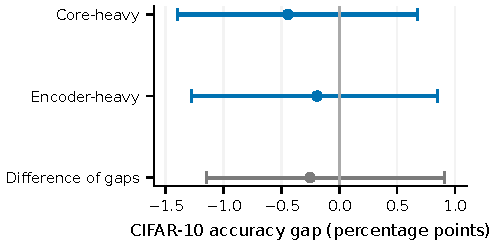
\includegraphics[width=0.66\linewidth]{figures/image_boundary.pdf}
\caption{\textbf{Natural-image scope boundary.} CIFAR-10 subset
accuracy minus the mean over 20 degree nulls, with original five-seed
paired bootstrap 95\% intervals. Both capacity regimes and their
difference include zero. The recurrent model uses reverse-directed
connectome support; this is not a test of forward biological visual
computation.}
\label{fig:image}
\end{figure}

\section{Executed MLP on the matched narrow graphs}
\label{sec:supp-mlp}
The subspace replay and the visual parity XOR use the archived readout and
the ten recorded seeds. The MLP is
$32\!\to\!64\!\to\!1$ with a ReLU, Adam at learning rate 0.006, binary
cross-entropy, and 120 epochs of 32 batches of 128. Evaluation uses 2,048
fresh samples. The linear control removes the hidden layer and keeps every
other choice. Sink features are $TX_{ab}$ for the reconstructed transfers.
Per-seed subspace MLP accuracies, in seed order, are
0.979, 0.969, 0.975, 0.979, 0.983, 0.958, 0.981, 0.984, 0.979, 0.977
for the base graph;
0.978, 0.970, 0.987, 0.978, 0.984, 0.967, 0.976, 0.988, 0.972, 0.990
for named-edge zero; and
0.501, 0.495, 0.491, 0.489, 0.489, 0.529, 0.506, 0.510, 0.537, 0.491
for path zero. Visual MLP accuracies in the same order are
0.685, 0.639, 0.684, 0.663, 0.666, 0.688, 0.648, 0.646, 0.650, 0.658;
0.748, 0.749, 0.752, 0.752, 0.757, 0.740, 0.733, 0.735, 0.754, 0.737; and
0.501, 0.504, 0.510, 0.497, 0.512, 0.497, 0.506, 0.510, 0.537, 0.491.
Every linear seed on both tasks falls between 0.473 and 0.539.

\section{Digit-field readout on the matched narrow graphs}
\label{sec:supp-fields}
The assay uses the reconstructed narrow $k{=}4$ base, named-edge zero, and
path-zero graphs. Incoming-normalized two-step transfer is recomputed from
each edge list and matches the source-to-sink matrices reported for these three graphs. In-degree
sequences, out-degree sequences, and module-pair counts agree across the
three graphs. The base common-relay pairs are $(9,4)$ and $(9,5)$; both
edited graphs have none. Column geometry is part of the recorded check:
the base columns are scalar multiples, the named-edge columns have cosine
$1/\sqrt{2}$, and the path-zero source-$b$ column is identically zero.

Digits are the 1,797 $8{\times}8$ images in the UCI optical digits
set, scaled by $1/16$. The upper field is rows $0$--$3$
and the lower field is rows $4$--$7$. Five stratified shuffles hold out 25\%
of the images. Independent pairing is a derangement inside the training
images and, separately, inside the test images, so no image or label crosses
the split. The readout is ridge least squares with weight penalty $10^{-4}$,
fit to the concatenated 64 sink features after training-set standardization.
The reported accuracy is this closed-form readout, not a selected training
epoch. Pixel $R^2$ uses the same features to predict the 32 held-out field
pixels.

\begin{table}[H]
\centering
\caption{\textbf{Per-split digit-field accuracies.} Independent lower- and
upper-field identity, then the intact digit. The pixel ceilings on these
splits average 0.933, 0.802, and 0.792 for the full image, upper field, and
lower field.}
\label{tab:field-splits}
\small
\begin{tabular}{@{}lccccccc@{}}
\toprule
Split & \multicolumn{3}{c}{Lower, independent} & \multicolumn{3}{c}{Intact digit} & Path upper \\
\cmidrule(lr){2-4}\cmidrule(lr){5-7}
 & Base & Named & Path & Base & Named & Path & \\
\midrule
0 & 0.518 & 0.800 & 0.107 & 0.853 & 0.938 & 0.787 & 0.787 \\
1 & 0.516 & 0.773 & 0.102 & 0.876 & 0.918 & 0.820 & 0.820 \\
2 & 0.529 & 0.778 & 0.100 & 0.844 & 0.933 & 0.811 & 0.811 \\
3 & 0.511 & 0.784 & 0.113 & 0.847 & 0.944 & 0.789 & 0.789 \\
4 & 0.489 & 0.784 & 0.102 & 0.840 & 0.931 & 0.804 & 0.804 \\
\bottomrule
\end{tabular}
\end{table}

On every split, named-edge intact accuracy equals the full-image pixel
ceiling and path-zero upper and intact accuracies equal the upper-field
ceiling. A \texttt{torch.nn.Linear} readout trained for 120 full-batch Adam
steps at learning rate 0.05 on the first split reproduces the ordering:
intact accuracies 0.891, 0.949, and 0.847, and independent lower-field
accuracies 0.529, 0.811, and 0.111 for base, named-edge, and path zero.

\section{Source assets and reproducibility boundary}

The source release is MaleCNS v1.0, minimum confidence 0.5. The annotation
and weight tables are publicly specified at the following stable resource
paths (under the \texttt{flyem-male-cns} Google Cloud bucket):
\begin{itemize}
\item \texttt{v1.0/connectome-data/flat-connectome/}\\
\texttt{body-annotations-male-cns-v1.0-minconf-0.5.feather}
\item \texttt{v1.0/connectome-data/flat-connectome/}\\
\texttt{connectome-weights-male-cns-v1.0-minconf-0.5.feather}
\end{itemize}
The corresponding source record is Berg et al., \emph{Cell}, 2026,
DOI: 10.1016/j.cell.2026.08.015. Recorded table sizes are 14,483,314
and 1,051,241,946 bytes. The extraction scripts read projected columns
in Arrow record batches rather than densifying the complete table.

The recovered original archive contains extraction/intervention code,
configurations, source hashes, per-seed accuracies, comparison families
and logged invariants, but lacked the small graph NPZs themselves.
We restored the source table and reconstructed those assets. The dense
base NPZ hashes are
\texttt{1a7fcf45bdf7607c...} (broad) and
\texttt{1100454a9740c907...} (narrow), exactly matching the frozen records.
Small reconstructed base and dose NPZs, full hashes, and source-to-sink
route terms are included in the supplied asset directory. Original
dose-instance hashes remain unavailable, so the distinction between
reconstructed inputs and historical trained executions is retained.

The supplied \texttt{evidence/source-manifest.json} identifies each copied
input by its original workspace-relative path and SHA-256. The
\texttt{analysis/observations.csv} file indexes all main path-study cells,
while the original JSON copies retain individual seeds and comparison
statistics. Archived-accuracy analysis and figure generation operate only on these copies
and do not retrain the archived models. The digit-field assay fits a new linear
readout on the reconstructed propagators, as specified above. The executed MLP
comparison, the CIFAR-10 identity assay, and the digit-identity comparison train new readouts on reconstructed
transfers; they do not reload archived weights. The CIFAR-10 encoder uses local training batches 2--4 because batch 1 is absent and batch 5 does not unpickle; the official test batch is held out. Full result matrices and tables, as well
as the reconstructed-graph transfer checks, can be regenerated from the
small supplied files. Rebuilding the graphs from scratch additionally
requires the public tables; reproducing historical trained readouts is
a separate operation that was not performed in this synthesis.

\end{document}
